% Intended LaTeX compiler: pdflatex
\documentclass[../main]{subfiles}


\begin{document}

\section{Percettrone}
\label{sec:org8e775fb}
Il modello di \href{20250624155858-neurone_artificiale.org}{neurone} più semplice è quello che riceve degli input, li somma dopo averli moltiplicati per dei pesi, e:
\begin{itemize}
\item restituisce \(0\) se la somma così ottenuta non supera un \uline{treshold} \(b\);
\item restituisce \(1\) se la somma così ottenuta è maggiore o uguale a \(b\).
\end{itemize}

Questo viene schematizzato in questo modo:
\begin{equation*}
\begin{tikzcd}[ampersand replacement=\&,cramped]
	{-1} \\
	{x_1} \\
	{x_2} \&\& {\boxed{\Sigma, H}} \&\& y \\
	\vdots \\
	{x_n}
	\arrow["b"{description}, from=1-1, to=3-3]
	\arrow["{w_1}"{description}, from=2-1, to=3-3]
	\arrow["{w_2}"{description}, from=3-1, to=3-3]
	\arrow[from=3-3, to=3-5]
	\arrow["{w_n}"{description}, from=5-1, to=3-3]
\end{tikzcd}
\end{equation*}
e l'output \(y\) è dato da\footnote{La funzione \(H:\R\to \R\) è la \href{20250624161413-funzione_di_heaviside.org}{Funzione di Heaviside}:
\begin{equation*}
H(x) = \begin{cases}
1 & x\ge 0\\
0 & x<0
\end{cases}
\end{equation*}}
\begin{equation*}
y=H\left(\sum_{i=0}^{n} x_{i}\,w_{i}\right)
\end{equation*}
dove per convenzione si è posto \(w_{0}=b\) e \(x_{0}=-1\).

La convenzione è per semplicità di notazione, infatti
\begin{equation*}
H\left(\sum_{i=0}^{n} x_{i}\,w_{i}\right)=\begin{cases}
1 & \sum_{i=1}^{n} x_{i}\, w_{i}\ge b\\
0 & \sum_{i=1}^{n} x_{i}\, w_{i}< b
\end{cases}
\end{equation*}

\begin{definizione}
Il \uline{percettrone} è il neurone con \href{20250624155858-neurone_artificiale.org}{funzione di attivazione} \(H\).
\end{definizione}
\subsection{Interpretazione Geometrica}
\label{sec:orgdc87b08}

Consideriamo il neurone con dimensione di input \(2\), ovvero \(\bm{x} = (x_{1},x_{2})\). Al variare di \(w_{1},w_{2},b\), l'output del neurone è quello mostrato in Figura~\ref{fig:outputperceptron}

\begin{figure}
\begin{center}
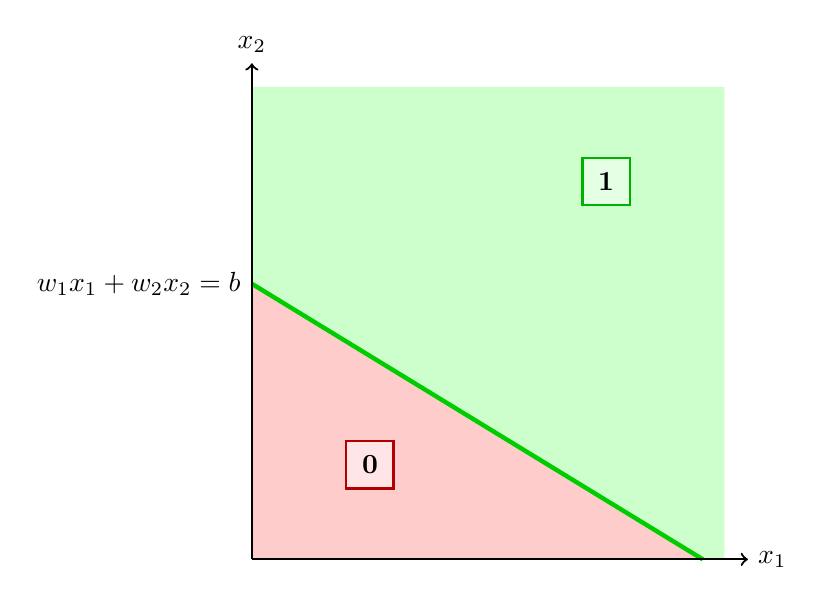
\begin{tikzpicture}[scale=3]

  % Parameters
  \def\wone{1.1}
  \def\wtwo{1.8}
  \def\b{2.1}

  % Define points for the line: w1*x1 + w2*x2 = b
  \coordinate (A) at (0, {(\b - \wone*0)/\wtwo}); % left
  \coordinate (B) at ({(\b - \wtwo*0)/\wone}, 0); % bottom

  % Intersection with box
  % \path[draw=green, ultra thick, name path=line] (A) -- (B);

  % Fill above the line (green)
  \fill[green!20] (0,2) -- (A) -- (B) -- (2,0) -- (2,2) -- cycle;

  % Fill below the line (red)
  \fill[red!20] (0,0) -- (2,0) -- (B) -- (A) -- cycle;

  % Line itself
  \draw[ultra thick, green!80!black] (A) node[left, black] {$w_1 x_1 + w_2 x_2 = b$} -- (B);

  % Boxed "1" in green region
  \node[draw=green!70!black, fill=green!10, thick, minimum size=6mm, anchor=center] at (1.5,1.6) {\bfseries 1};

  % Boxed "0" in red region
  \node[draw=red!70!black, fill=red!10, thick, minimum size=6mm, anchor=center] at (0.5,0.4) {\bfseries 0};

  % Axes and grid
  \draw[->, thick] (0,0) -- (2.1,0) node[right] {$x_1$};
  \draw[->, thick] (0,0) -- (0,2.1) node[above] {$x_2$};
\end{tikzpicture}
\end{center}
\caption{\label{fig:outputperceptron}Output di un Percettrone}
\end{figure}

Inoltre:
\begin{itemize}
\item il percettrone sa implementare la funzione \href{20250710120853-and_logico.org}{AND}
\begin{center}
\begin{tabular}{c c c}
\hline
\(x_{1}\) & \(x_{2}\) & AND\\
\hline
0 & 0 & 0\\
0 & 1 & 0\\
1 & 0 & 0\\
1 & 1 & 1\\
\hline
\end{tabular}
\end{center}
con parametri \(w_{1}=w_{2}=1\) e \(b=1.5\), come in figura~\ref{per:and}

\item il percettrone sa implementare la funzione \href{20250710120858-or_logico.org}{OR}
\begin{center}
\begin{tabular}{c c c}
\hline
\(x_{1}\) & \(x_{2}\) & OR\\
\hline
0 & 0 & 0\\
0 & 1 & 1\\
1 & 0 & 1\\
1 & 1 & 1\\
\hline
\end{tabular}
\end{center}
con parametri \(w_{1}=w_{2}=1\) e \(b=0.5\), come in figura~\ref{per:and}
\item il percettrone \uline{non sa} implementare la funzione \href{20250710120916-xor_logico.org}{XOR}, mostrata in figura~\ref{per:xor}
\begin{center}
\begin{tabular}{c c c}
\hline
\(x_{1}\) & \(x_{2}\) & XOR\\
\hline
0 & 0 & 0\\
0 & 1 & 1\\
1 & 0 & 1\\
1 & 1 & 0\\
\hline
\end{tabular}
\end{center}
Infatti, supponiamo che esistano \(w_{1},w_{2},b \in\R\) tale che la retta \(w_{1}x_{1}+w_{2}x_{2}\) è
\begin{align*}
  \set{(0,1),(1,0)}\quad &\ge b\\
  \set{(0,0),(1,0)}\quad &<b
\end{align*}
allora \(w_{2}\ge b\) e \(w_{1}\ge b\) per la prima espressione, ma \(w_{1}<b\) per la seconda. Assurdo.
\end{itemize}


\begin{figure}
\begin{center}
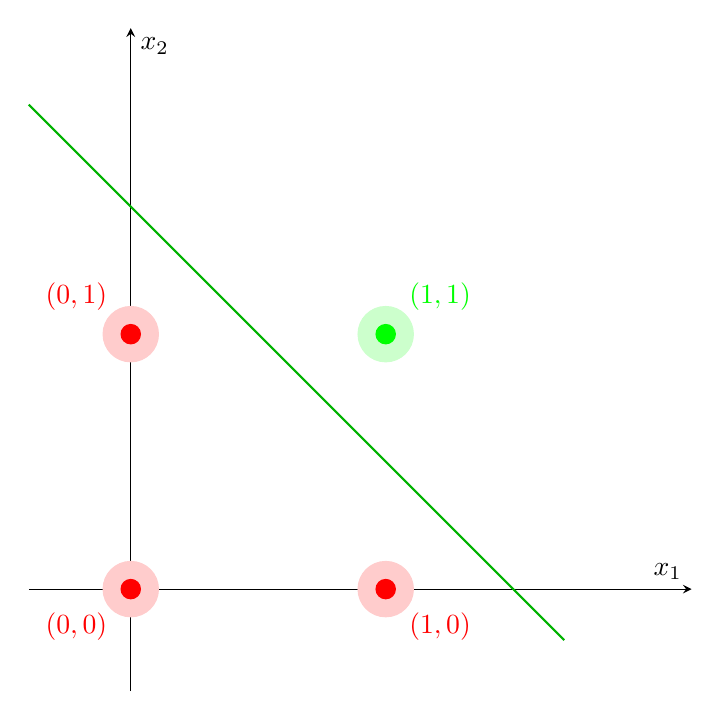
\begin{tikzpicture}
  % Definisci i parametri w1, w2, b qui:
  \def\wone{1}
  \def\wtwo{1}
  \def\b{1.5}

  \begin{axis}[
    axis lines=middle,
    xmin=-0.4, xmax=2.2,
    ymin=-0.4, ymax=2.2,
    xlabel={$x_1$},
    ylabel={$x_2$},
    width=10cm,
    height=10cm,
    ticks=none,
    enlargelimits=false,
    clip=false,
  ]

    % Retta: x2 = (b - w1*x1)/w2
    \addplot[domain=-0.4:1.7, samples=200, thick, green!70!black]
      { (\b - \wone*x)/\wtwo };

    % Punti singoli

    % (0,0)
    \addplot[only marks, mark=*, mark size=10pt, red!20] coordinates {(0,0)};
    \addplot[only marks, mark=*, mark size=3.5pt, red] coordinates {(0,0)} node [below left, xshift=-5pt, yshift=-5pt] {$(0,0)$};

    % (0,1)
    \addplot[only marks, mark=*, mark size=10pt, red!20] coordinates {(0,1)};
    \addplot[only marks, mark=*, mark size=3.5pt, red] coordinates {(0,1)} node [above left, xshift=-5pt, yshift=5pt] {$(0,1)$};

    % (1,0)
    \addplot[only marks, mark=*, mark size=10pt, red!20] coordinates {(1,0)};
    \addplot[only marks, mark=*, mark size=3.5pt, red] coordinates {(1,0)} node [below right, xshift=5pt, yshift=-5pt] {$(1,0)$};

    % (1,1)
    \addplot[only marks, mark=*, mark size=10pt, green!20] coordinates {(1,1)};
    \addplot[only marks, mark=*, mark size=3.5pt, green] coordinates {(1,1)} node [above right, xshift=5pt, yshift=5pt] {$(1,1)$};

  \end{axis}
\end{tikzpicture}
\end{center}
\caption{\label{per:and}Funzione AND}
\end{figure}

\begin{figure}
\begin{center}
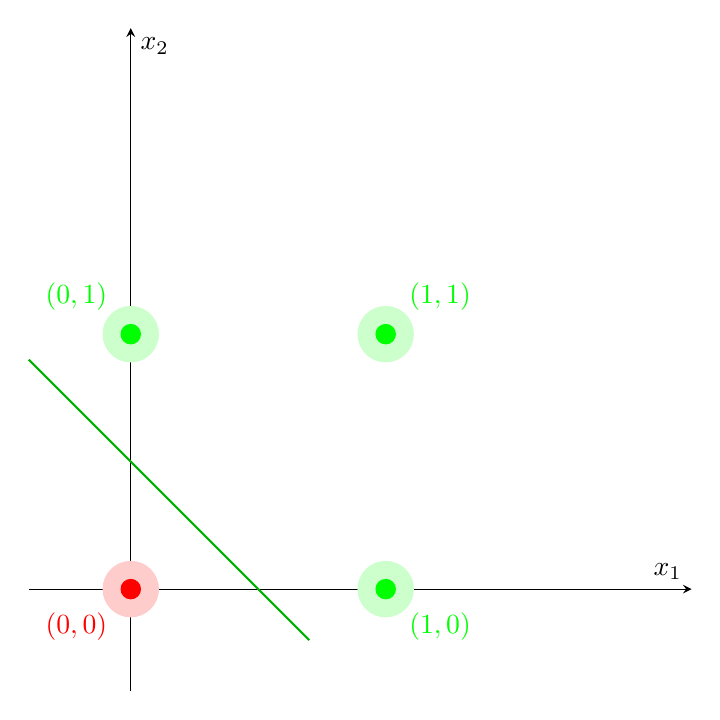
\begin{tikzpicture}
  % Definisci i parametri w1, w2, b qui:
  \def\wone{1}
  \def\wtwo{1}
  \def\b{0.5}

  \begin{axis}[
    axis lines=middle,
    xmin=-0.4, xmax=2.2,
    ymin=-0.4, ymax=2.2,
    xlabel={$x_1$},
    ylabel={$x_2$},
    width=10cm,
    height=10cm,
    ticks=none,
    enlargelimits=false,
    clip=false,
  ]

    % Retta: x2 = (b - w1*x1)/w2
    \addplot[domain=-0.4:0.7, samples=200, thick, green!70!black]
      { (\b - \wone*x)/\wtwo };

    % Punti singoli

    % (0,0)
    \addplot[only marks, mark=*, mark size=10pt, red!20] coordinates {(0,0)};
    \addplot[only marks, mark=*, mark size=3.5pt, red] coordinates {(0,0)} node [below left, xshift=-5pt, yshift=-5pt] {$(0,0)$};

    % (0,1)
    \addplot[only marks, mark=*, mark size=10pt, green!20] coordinates {(0,1)};
    \addplot[only marks, mark=*, mark size=3.5pt, green] coordinates {(0,1)} node [above left, xshift=-5pt, yshift=5pt] {$(0,1)$};

    % (1,0)
    \addplot[only marks, mark=*, mark size=10pt, green!20] coordinates {(1,0)};
    \addplot[only marks, mark=*, mark size=3.5pt, green] coordinates {(1,0)} node [below right, xshift=5pt, yshift=-5pt] {$(1,0)$};

    % (1,1)
    \addplot[only marks, mark=*, mark size=10pt, green!20] coordinates {(1,1)};
    \addplot[only marks, mark=*, mark size=3.5pt, green] coordinates {(1,1)} node [above right, xshift=5pt, yshift=5pt] {$(1,1)$};

  \end{axis}
\end{tikzpicture}
\end{center}
\caption{\label{per:or}Funzione OR}
\end{figure}

\begin{figure}
\begin{center}
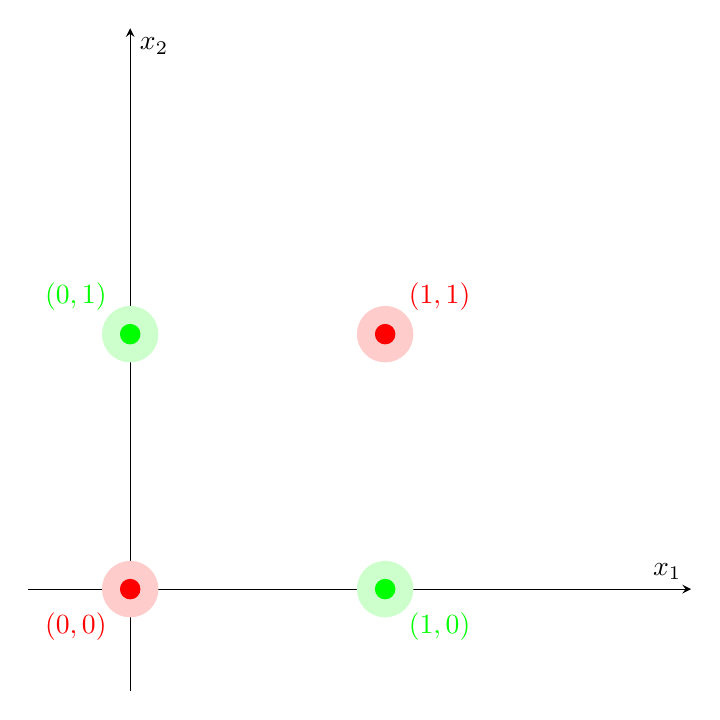
\begin{tikzpicture}
  % Definisci i parametri w1, w2, b qui:
  \def\wone{1}
  \def\wtwo{1}
  \def\b{0.5}

  \begin{axis}[
    axis lines=middle,
    xmin=-0.4, xmax=2.2,
    ymin=-0.4, ymax=2.2,
    xlabel={$x_1$},
    ylabel={$x_2$},
    width=10cm,
    height=10cm,
    ticks=none,
    enlargelimits=false,
    clip=false,
  ]

    % Punti singoli

    % (0,0)
    \addplot[only marks, mark=*, mark size=10pt, red!20] coordinates {(0,0)};
    \addplot[only marks, mark=*, mark size=3.5pt, red] coordinates {(0,0)} node [below left, xshift=-5pt, yshift=-5pt] {$(0,0)$};

    % (0,1)
    \addplot[only marks, mark=*, mark size=10pt, green!20] coordinates {(0,1)};
    \addplot[only marks, mark=*, mark size=3.5pt, green] coordinates {(0,1)} node [above left, xshift=-5pt, yshift=5pt] {$(0,1)$};

    % (1,0)
    \addplot[only marks, mark=*, mark size=10pt, green!20] coordinates {(1,0)};
    \addplot[only marks, mark=*, mark size=3.5pt, green] coordinates {(1,0)} node [below right, xshift=5pt, yshift=-5pt] {$(1,0)$};

    % (1,1)
    \addplot[only marks, mark=*, mark size=10pt, red!20] coordinates {(1,1)};
    \addplot[only marks, mark=*, mark size=3.5pt, red] coordinates {(1,1)} node [above right, xshift=5pt, yshift=5pt] {$(1,1)$};

  \end{axis}
\end{tikzpicture}
\end{center}
\caption{\label{per:xor}Funzione XOR}
\end{figure}
\subsection{Generalizzazione: classificazione binaria}
\label{sec:org2165c68}

Si consideri un percettrone con input bidimensionale, \(n=2\), e \(x,y \in [0,1]\).

Lo spazio dei possibili input è rappresentato da \([0,1]\times [0,1]\). Si supponga che sia diviso in due: \(\mathcal{G}_{1}, \mathcal{G_{2}}\), e che vi sia una funzione \(z(x,y) \in \set{0,1}\) che indica l'appartenenza ad uno dei due gruppi.

Si vuole studiare se il percettrone è in grado di distinguere gli elementi del gruppo 1 da quelli del gruppo 2. Sia \(f_{\bm{w},b}(x,y)\) l'output del percettrone.

Si conoscesse esattamente \(z(x,y)\) sarebbe possibile calcolare i pesi \(\bm{w}=(w_{1},w_{2})\) e \(b\) minimizzando la norma \(L^{2}\):\footnote{Vedi ``\href{20250710140734-valore_atteso.org}{Valore atteso}''}
\begin{equation*}
C(\bm{w},b) = \int_{[0,1]^{2}}\left(f_{\bm{w},b}(x,y)-z(x,y)\right)^{2}\dif x\dif y = \media\left[{(f_{\bm{w},b}(x,y)-z(x,y))^{2}}\right]
\end{equation*}
Questo è quindi il metodo del \href{20250710141709-mean_square_error.org}{Mean Square Error} (MSE)

\uline{Senza conoscere esattamente \(\mathcal{G}_{1}\) e \(\mathcal{G}_{2}\)}, ma conoscendo soltanto la classificazione di un numero finito di punti
\begin{equation*}
\set{\langle(x_{i},y_{i}), z_{i} = z(x_{i},y_{i})\rangle\mid i=1,\dots,N}
\end{equation*}
è possibile soltanto calcolare la versione empirica \(\tilde{C}(\bm{w},b)\), utilizzando la \href{20250710140836-legge_dei_grandi_numeri.org}{legge dei grandi numeri}:
\begin{equation*}
\tilde{C}(\bm{w},b) = \frac{1}{N}\sum_{i=1}^{N}\left(f_{\bm{w},b}(x_{i},y_{i})-z_{i}\right)^{2}\hspace{1em} \xrightarrow[N\to\infty]{}\hspace{1em} C(\bm{w},b)
\end{equation*}
Questo è il metodo dell'\href{20250710141709-mean_square_error.org}{Empirical MSE}.
\subsection{Perceptron Learning Algorithm}
\label{sec:orge8efa60}
Sia \(D=\set{(\bm{x}_{i},y_{i})\mid i =1,\dots,N}\), con \(z_{i} \in \set{0,1}\) l'insieme su cui si esegue l'allenamento, e sia \(f_{\bm{w}}(\bm{x})=\varphi(\bm{w}\cdot \bm{x})\) la funzione di output di un neurone \hyperref[sec:org8e775fb]{perceptron}.

Si definiscono
\begin{align*}
P&\coloneqq \set{\bm{x}\mid (\bm{x},1) \in D}\\
N&\coloneqq \set{\bm{x} \mid (\bm{x},0) \in D}
\end{align*}

Si vuole trovare \(\bm{w}^{*}\) tale per cui
\begin{align*}
\forall \bm{x} \in P:\quad f_{\bm{w}^{*}}(\bm{x}) &=1\\
\forall \bm{x} \in N:\quad f_{\bm{w}^{*}}(\bm{x}) &=0
\end{align*}

L'\href{20250627110009-training_error_and_test_error.org}{algoritmo di apprendimento} per questo task è il seguente: si scelga \(\bm{w}^{(0)}\) casualmente. Il seguente ciclo iterativo si esegue finché non c'è convergenza: al passo \(k+1\), si scelga casualmente \(\bm{x} \in P\cup N\);
\begin{itemize}
\item se \(\bm{x} \in P\) e \(\bm{w}^{(k)}\cdot \bm{x} <0\) allora si pone \(\bm{w}^{(k+1)} \coloneqq \bm{w}^{(k)}+\bm{x}\);
\item se \(\bm{x} \in N\) e \(\bm{w}^{(k)}\cdot \bm{x} \ge 0\) allora si pone \(\bm{w}^{(k+1)} \coloneqq \bm{w}^{(k)}-\bm{x}\);
\item altrimenti si pone \(\bm{w}^{(k+1)}=\bm{w}^{(k)}\).
\end{itemize}

In sostanza l'algoritmo è riassumibile come segue: fissato \(\bm{w}^{(0)}\) e una \href{20250115100904-successione.org}{successione} di punti \((\bm{x}_{i})_{i \in \N} \subseteq P\cup N\) catalogati da \(y_{i}\)\footnote{Ovvero per ogni \(i \in \N\), \((\bm{x}_{i},y_{i}) \in D\).}, si ha che
\begin{equation*}
\bm{w}^{(k+1)} \coloneqq \bm{w}^{(k)} + \left(y_{k} - \varphi(\bm{w}^{(k)}\cdot\bm{x}_{k})\right)\cdot\bm{x}_{k}.
\end{equation*}

\begin{oss}
Quando tutti gli elementi di \(P\cup N\) sono stati processati dall'algoritmo (e dunque si ricomincia a sceglierli), si dice che è passata un'epoca.
\end{oss}
\begin{thm}
Se il dataset è linearmente separabile allora il percettrone trova un iperpiano di separazione in un numero finito di passi, altrimenti cicla infinite volte.
\end{thm}
\begin{proof}
Se il training set \(\mathscr{T}\) è separabile linearmente, allora esiste \(\bm{w}^{*}\) tale che
\begin{equation*}
\forall (\bm{x}^{i},y_{i}) \in \mathscr{T}:\qquad y_{i} = \varphi(\bm{w}^{*}\cdot \bm{x}^{i}).
\end{equation*}
Si noti che in \(\bm{w}^{*}\) è presente sempre il bias.

Si riscala il tutto in maniera tale che
\begin{itemize}
\item \(\norma{\bm{w}^{*}} = 1\);
\item \(\forall (\bm{x}^{i},y_{i}) \in \mathscr{T}\): \(\norma{\bm{x}^{i}}\le 1\).
\end{itemize}

Sia quindi
\begin{equation*}
\gamma \coloneqq \min_{(\bm{x}, y) \in \mathscr{T}} |\bm{w}^{*}\cdot\bm{x}|.
\end{equation*}

Sia \(\bm{w}^{(0)} = \bm{0}\), sia inoltre \((\bm{w}^{(k)})_{k \in \N}\) la successione di pesi costruita con l'algoritmo. Si supponga di aver eliminato tutti i termini uguali, tranne l'eventuale coda dettata dalla convergenza.

Allora valgono le seguenti disuguaglianze (dimostrate in fondo):
\begin{align}
\text{se }\bm{w}^{(k+1)}\neq \bm{w}^{(k)}\text{:}\hspace{3em}\bm{w}^{(k+1)}\cdot \bm{w}^{*}&\ge \bm{w}^{(k)}\cdot\bm{w}^{*} + \gamma;\label{perc:dis:1}\\
\bm{w}^{(k+1)}\cdot \bm{w}^{(k+1)} &\le \bm{w}^{(k)}\cdot \bm{w}^{(k)} + 1.\label{perc:dis:2}
\end{align}

Applicando iterativamente \eqref{perc:dis:1}, si ottiene che, se per ogni \(i< k\) si ha \(\bm{w}^{(i+1)}\neq \bm{w}^{(i)}\), allora
\begin{equation}
\bm{w}^{(k)}\cdot \bm{w}^{*} \ge \bm{w}^{(k-1)}\cdot\bm{w}^{*} + \gamma\ge (\bm{w}^{(k-2)}\cdot\bm{w}^{*} +\gamma) + \gamma\ge \dots \ge \bm{w}^{(0)}\cdot\bm{w}^{*} + k\gamma = k\gamma.\label{perc:dis:3}
\end{equation}
mentre applicando iterativamente \eqref{perc:dis:2}, si ottiene
\begin{equation*}
\bm{w}^{(k)}\cdot \bm{w}^{(k)} \le \bm{w}^{(k-1)}\cdot \bm{w}^{(k-1)} +1\le \dots\le \bm{w}^{(0)}\cdot\bm{w}^{(0)} + k = k
\end{equation*}
Quest'ultima disuguaglianza si utilizza per dimostrare:
\begin{equation}
\bm{w}^{(k)}\cdot \bm{w}^{*} = \norma{\bm{w}^{(k)}}\cdot \parentesi{=1}{\norma{\bm{w}^{*}}}\cdot\cos\theta\le \norma{\bm{w}^{(k)}} = \sqrt{\bm{w}^{(k)}\cdot \bm{w}^{(k)}}\le\sqrt{k}
\label{perc:dis:4}
\end{equation}

Combinando dunque \eqref{perc:dis:3} e \eqref{perc:dis:4} si ottiene che, se per ogni \(i< k\) si ha \(\bm{w}^{(i+1)}\neq \bm{w}^{(i)}\), allora
\begin{equation*}
k\gamma \le \bm{w}^{(k)}\cdot \bm{w}^{*}\le \sqrt{k}.
\end{equation*}
Essendo tutte quantità positive, si ottiene \(k^{2}\gamma^{2}\le k\), ovvero
\begin{equation*}
k\le\frac{1}{\gamma^{2}}.
\end{equation*}

Si è quindi dimostrato che se \(k>1/\gamma^{2}\) allora esiste \(i<k\) tale che \(w^{(i+1)}=w^{(i)}\). Per costruzione, quindi, l'algoritmo converge ad un certo valore \(\bm{w}\), che per costruzione separa i punti.
\end{proof}
\end{document}
